\section{Keystone Enclave}
%todo modificare questa intro
Device manufacturers are now taking security concerns more seriously than they previously did as a result of the rise in the popularity of networked devices in recent years.
To adequately address these challenges, Trusted Execution Environments have been developed that define a way to ensure the integrity and confidentiality of sensitive data in the device that implements the specification \cite{IntroTEE}. Keystone \cite{lee2020keystone} is an open-source framework for creating RISC-V hardware-based Trusted Execution Environments that are adaptable for use on a variety of platforms. 

\subsection{Trusted Execution Environment}
A Trusted Execution Environment (TEE) is a safe area within a CPU. It runs in an isolated environment and in parallel with the operating system.
It ensures that the confidentiality and integrity of the code and data loaded in the TEE are preserved. 
Trusted applications running on TEE have access to the full capabilities of a device's main processor and memory, while hardware isolation shields these components from user-installed apps running in the main operating system. The various included trusted applications are protected from one another by software and cryptographic isolations within the TEE \cite{IntroTEE}.
The two most common TEE implementations at the moment are ARM TrustZone and Intel SGX. All these TEEs make design decisions based on either the target applications or threat models and these choices are fixed since they are strictly hardware related. They were not designed to have flexibility or extensibility for enclave developers.  If the hardware changes or has a new feature, the enclave developer has to redesign the TEE.
All TEE platforms aim to reduce the enclave's Trusted computing Base, yet they have managed to achieve different degrees of success \cite{keysyone-blog-1}. The Trusted Computing Base (TCB) is a section of the system, it could include hardware, firmware and software, which is responsible for enforcing the security policy of the system \cite{tcb-def}. Additionally, closed-source hardware and microcode implementations make it impossible for a third party to evaluate the security of TEEs.

\subsection{Customizable Trusted Execution Environment}
Customizable TEE is the solution to these problems. It has been designed to be flexible, and configurable and to have a small TCB. It has been designed with clear abstractions and a modular programming model which simplifies for others to extend and add features to the TEE. A customizable TEE is Keystone \cite{lee2020keystone}. Three logical actors, such as the manufacturer (who makes the hardware), the platform provider (runs the hardware, such as a cloud provider), and the enclave developer (who writes software that runs in the enclaves), were identified by keystone developers as being a part of the customizable TEE ecosystem. In a customizable TEE, as opposed to a standard TEE, decisions made by all 3 actors together determine the security guarantees offered and the functionalities enabled \cite{keysyone-blog-1}. 
Keystone offers security primitives that can be joined together via the software framework rather than creating a single instance of TEE hardware. The TEE can be modified by the creator of the enclave and the platform provider to suit their threat models or platform configurations. The Keystone project offers a general and formally proven interface for a variety of devices to create an open standard for TEEs. 

\subsection{RISC-V Background}

\subsection{Keystone overview}


\begin{figure}[h!]
    \centering
    \includesvg[inkscapelatex=false, scale=0.40]{./chapters/images/TEE-keystone-vs-x86.svg}
    \caption{Architecture differences between x86 and keystone}
    \label{keystone-vs-x86}
\end{figure}

\begin{figure}[h!]
    \centering
    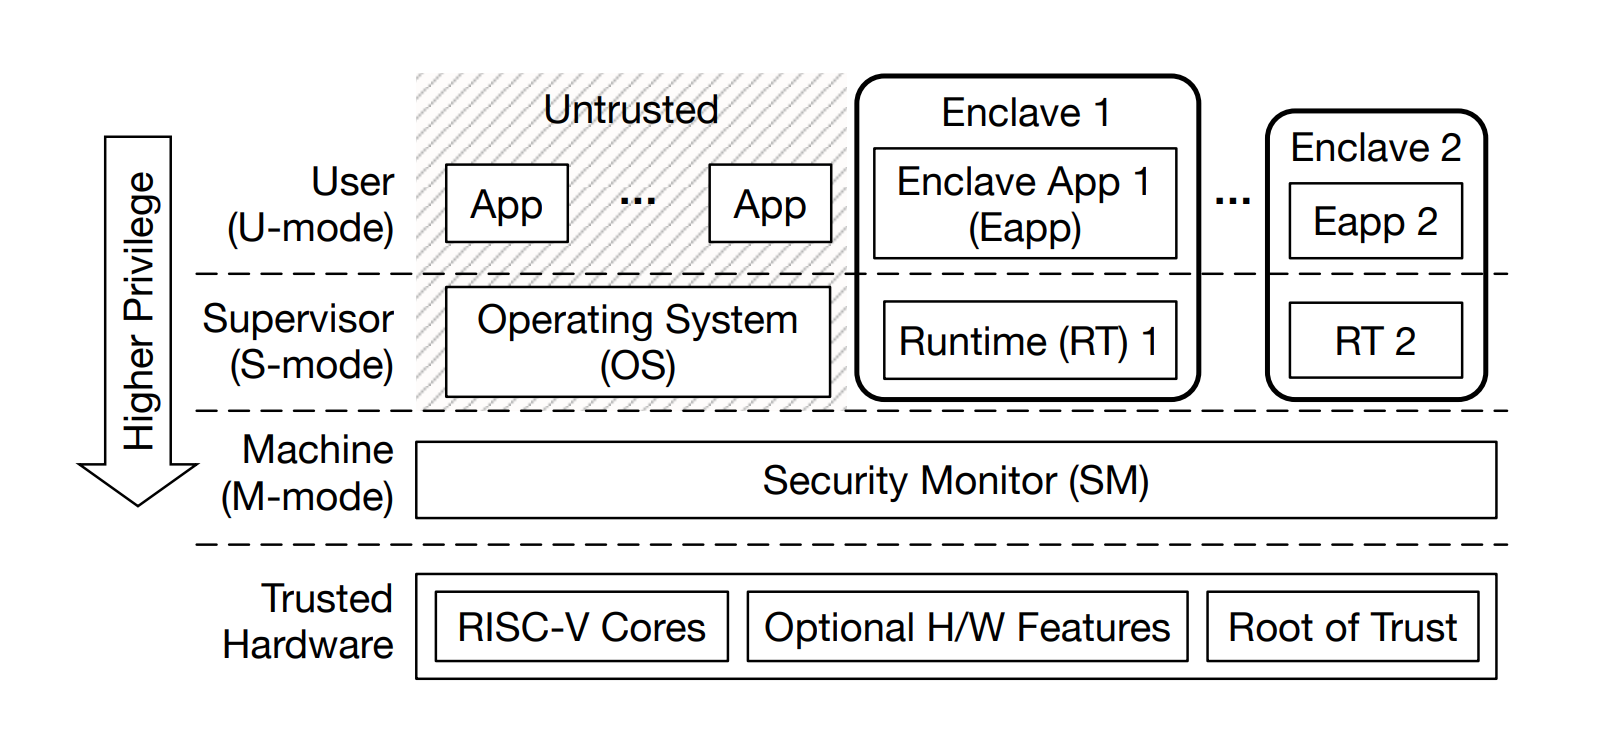
\includegraphics[scale=0.35]{./chapters/images/keystone-components.png}
    \caption{Keystone system with host processes, untrusted OS, security monitor, and multiple enclaves (each with runtime and eapp) \cite{lee2020keystone}.}
    \label{keystoneComponents}
\end{figure}
\subsubsection{Security Monitor}
\subsubsection{Runtime}